\section{Coupled geographic cost alternatives}
\subsection{A probability sample with an independently known control}
Each alternative climate member now drives sea-level components and a coastal
cost calculation. We retain the original 200 elevation bins, annual cash flows,
SSP4 OECD economics and the paired no-rise baseline. Sea-level change is uniform
across coasts because the target fingerprint and land-motion inputs have not
been recovered. Economic response parameters remain fixed at their declared
central values. Thus this experiment propagates the sampled climate and sea-level
variation but not the full target scientific or socioeconomic uncertainty.

The complete 9,531-coast calculation under a prescribed 1 m path supplies an
auxiliary cost $x_i$ and exact regional sum $X_r$. We sample coastal units
independently within seven World Bank regions and an unmapped stratum, assigning
\begin{equation}
 p_i=0.9\frac{|x_i|}{\sum_{k\in r}|x_k|}+\frac{0.1}{N_r}.
\end{equation}
Here $N_r$ is the number of eligible coasts in the stratum. All coasts have
positive inclusion probability. For a new path's cost $y_i$, we estimate
\begin{equation}
 \widehat Y_r=\beta X_r+\frac{1}{n_r}\sum_{j=1}^{n_r}
 \frac{y_{I_j}-\beta x_{I_j}}{p_{I_j}},
 \qquad \beta=\frac{S(2100)-S(2010)}{1\,{\rm m}}.
\end{equation}
The sampled indices $I_j$ are independent draws with replacement. Taking the
expectation cancels the control term and gives $\sum_i y_i$ for any fixed
$\beta$. This identity does not assume that coastal costs are linear in sea
level. The sample variance of the summands, divided by $n_r$, estimates the
conditional numerical variance. Variances add across independent strata;
using the same coasts for every climate member induces covariance between
their numerical errors.

Exact enumeration tests verify the estimator and its variance for a finite
three-coast population. A further 5,000 design replicates per test compare
estimates with complete independent 0.5, 1 and 2 m calculations. Biases lie
within 1.84 Monte Carlo standard errors, and empirical-to-estimated variance
ratios span 0.966--1.027. Normal 95\% intervals cover only 93.3--94.0\% at
sixteen draws per stratum. The variance check therefore supports the numerical
error estimate without establishing exact normal-interval coverage.

A six-path pilot covers the minimum and maximum sea-level paths and each
occupied warming category. Doubled flood quadrature changes selected cost by
less than $2\times10^{-16}$ relatively and preserves all tested policies.
The full calculation uses sixteen draws per stratum, 119 distinct coasts and
250 climate members: 29,750 climate--coast combinations. It takes 3,016 wall
seconds, including controlled pauses for serial validation. Median conditional
global cost SE is 6.26\% of estimated cost; the maximum is 9.22\%.

\subsection{Global distributions and comparison limits}
Figure~\ref{fig:coupledcost} shows the warming-conditioned cost estimates.
Under 50\% budget weights, the four median incremental costs are 0.208, 0.290,
0.664 and 1.217 trillion 2019 USD PPP. The corresponding 5th--95th ranges are
0.137--0.260, 0.214--0.440, 0.385--0.965 and 0.808--1.609 trillion. The highest
category contains only five members, with conditional ESS 4.23; its plotted
percentiles identify order statistics, not converged tail estimates.

The target reports medians of 1.2, 1.5, 2.1 and 2.6 trillion 2010 USD over a
2150 horizon. Our estimates are numerically smaller, but the monetary inputs,
reference-cost subtraction and time horizon differ. Applying the independently
documented CPI factor 0.852924 lowers the alternative values further; that
price-year conversion does not reconcile international PPP, exposure or
accounting. We do not report the remaining difference as a commensurate model
error. The target's threshold probabilities also differ substantially from
our alternative weights (published Table 1 and the figure inventory).

\begin{figure}[htbp]
\centering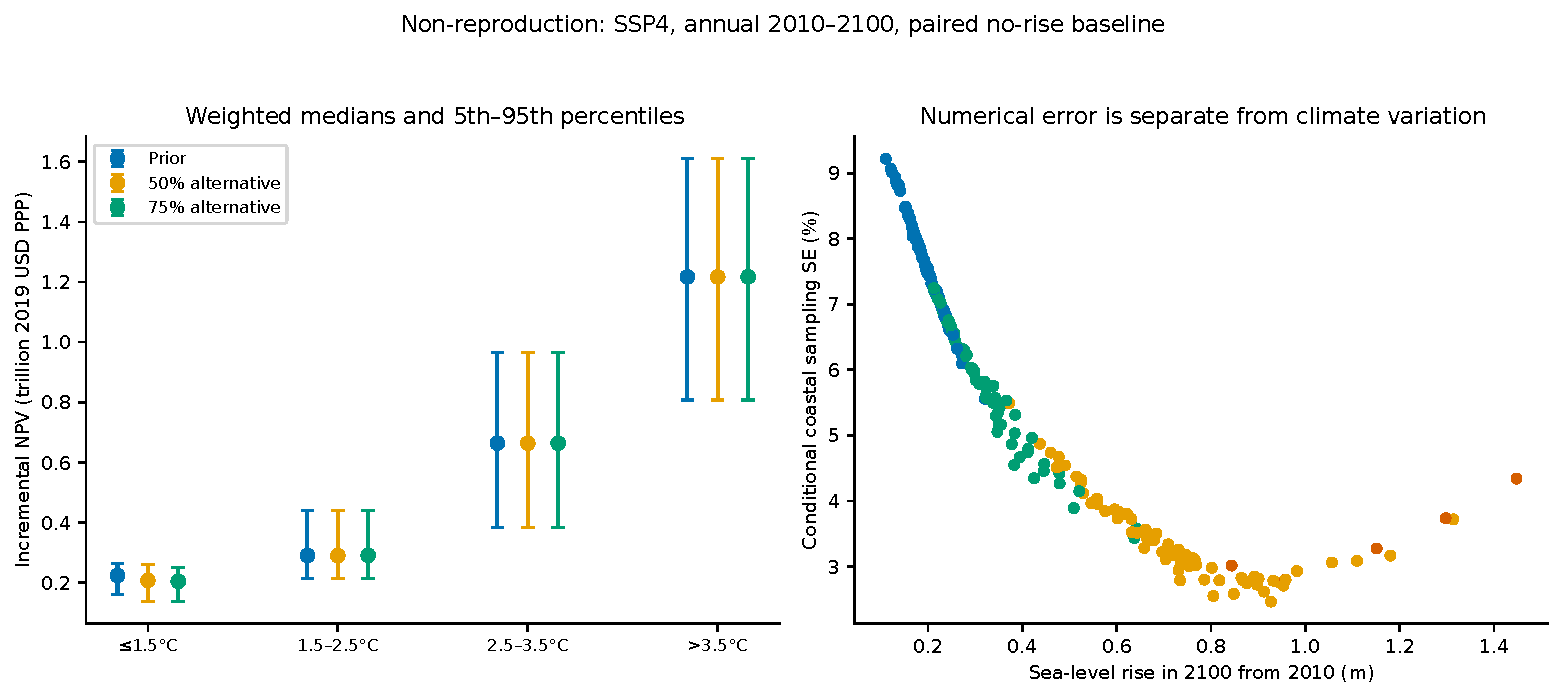
\includegraphics[width=\linewidth]{figures/coupled_coastal_cost_alternative.pdf}
\caption{Global cost alternatives corresponding to the quantities in main
Figure 1. Left: weighted medians and 5th--95th order statistics under three
emissions probability measures. Costs use annual 2010--2100 accounting, 4\%
discounting to 2010, 2019 USD PPP and a paired no-rise counterfactual. Right:
conditional coast-sampling SE for each climate member, separate from the
variation shown on the left. Errors are correlated across members because
coast draws are shared. Only five members occupy the highest warming category;
its tail percentiles remain unresolved. These are non-reproductions.}
\label{fig:coupledcost}
\end{figure}

\begin{figure}[htbp]
\centering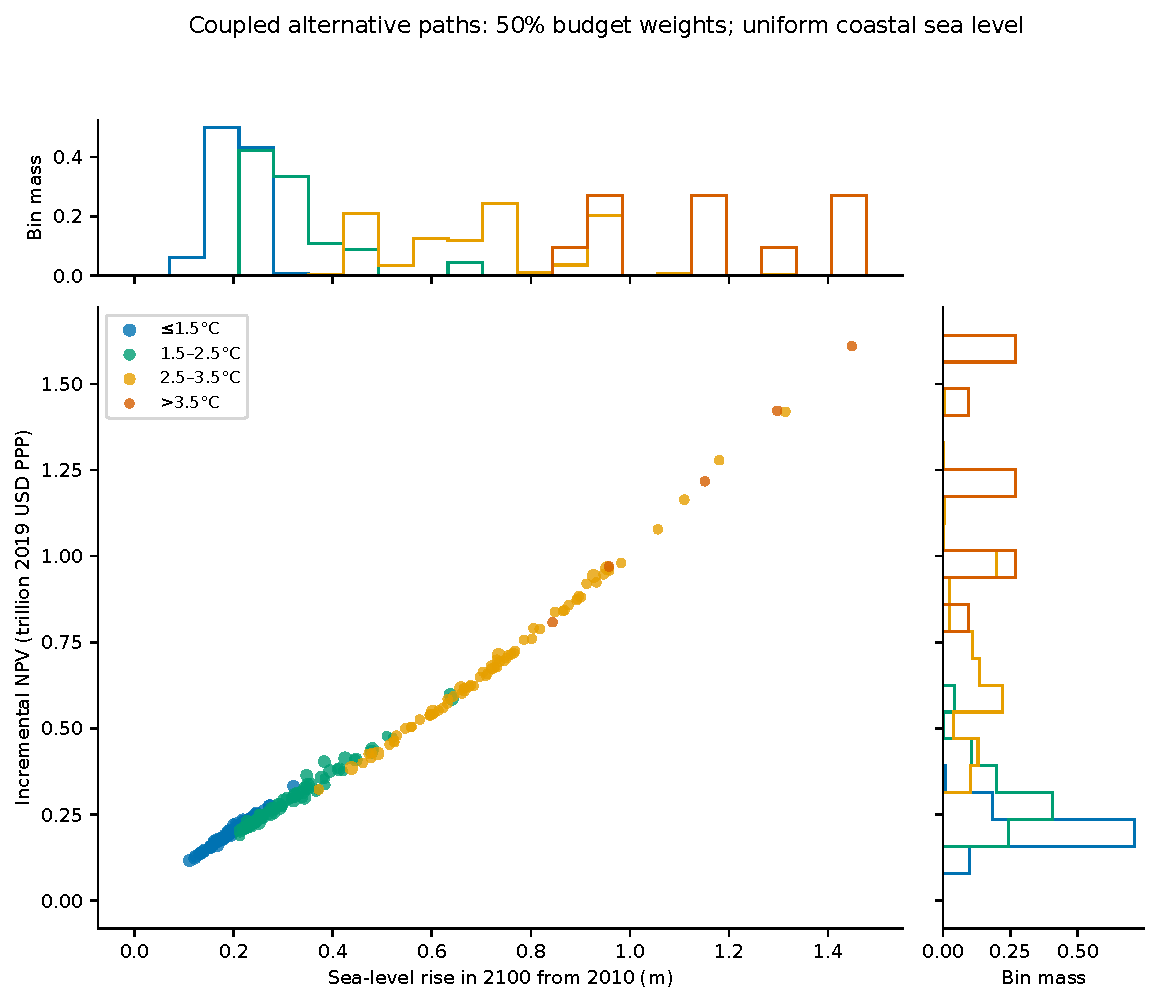
\includegraphics[width=.9\linewidth]{figures/coupled_coastal_joint_alternative.pdf}
\caption{Coupled sea level and coastal cost with empirical conditional
marginals, corresponding to main Figure 2. Symbol area reflects 50\% budget
weights and color identifies annual 2100 warming. Marginal histograms normalize
within each warming category and do not invent a smooth tail density. Sea level
is relative to 2010; its separate 1995--2014 transformation is documented in
Figure~\ref{fig:seaar6}. Coastal units, accounting and uncertainty differ from
the target, so the plotted relationship is an independent alternative.}
\label{fig:coupledjoint}
\end{figure}

\subsection{Regional burdens and planned movement}
The regional ranking differs from the target's written interpretation.
For category 3, East Asia and the Pacific has a median burden 0.591 percentage
points above the covered global cost/GDP ratio. Latin America and the Caribbean,
South Asia and Sub-Saharan Africa instead lie 0.218, 0.132 and 0.187 percentage
points below it. The target identifies disproportionate burdens across several
Global South regions. Agreement in the direction of increasing global costs
with warming therefore does not establish agreement in geographic inequality.
The denominator is independently acquired 2010 regional GDP in 2019 PPP units;
unmapped costs are excluded consistently from the covered global comparator.

\begin{figure}[htbp]
\centering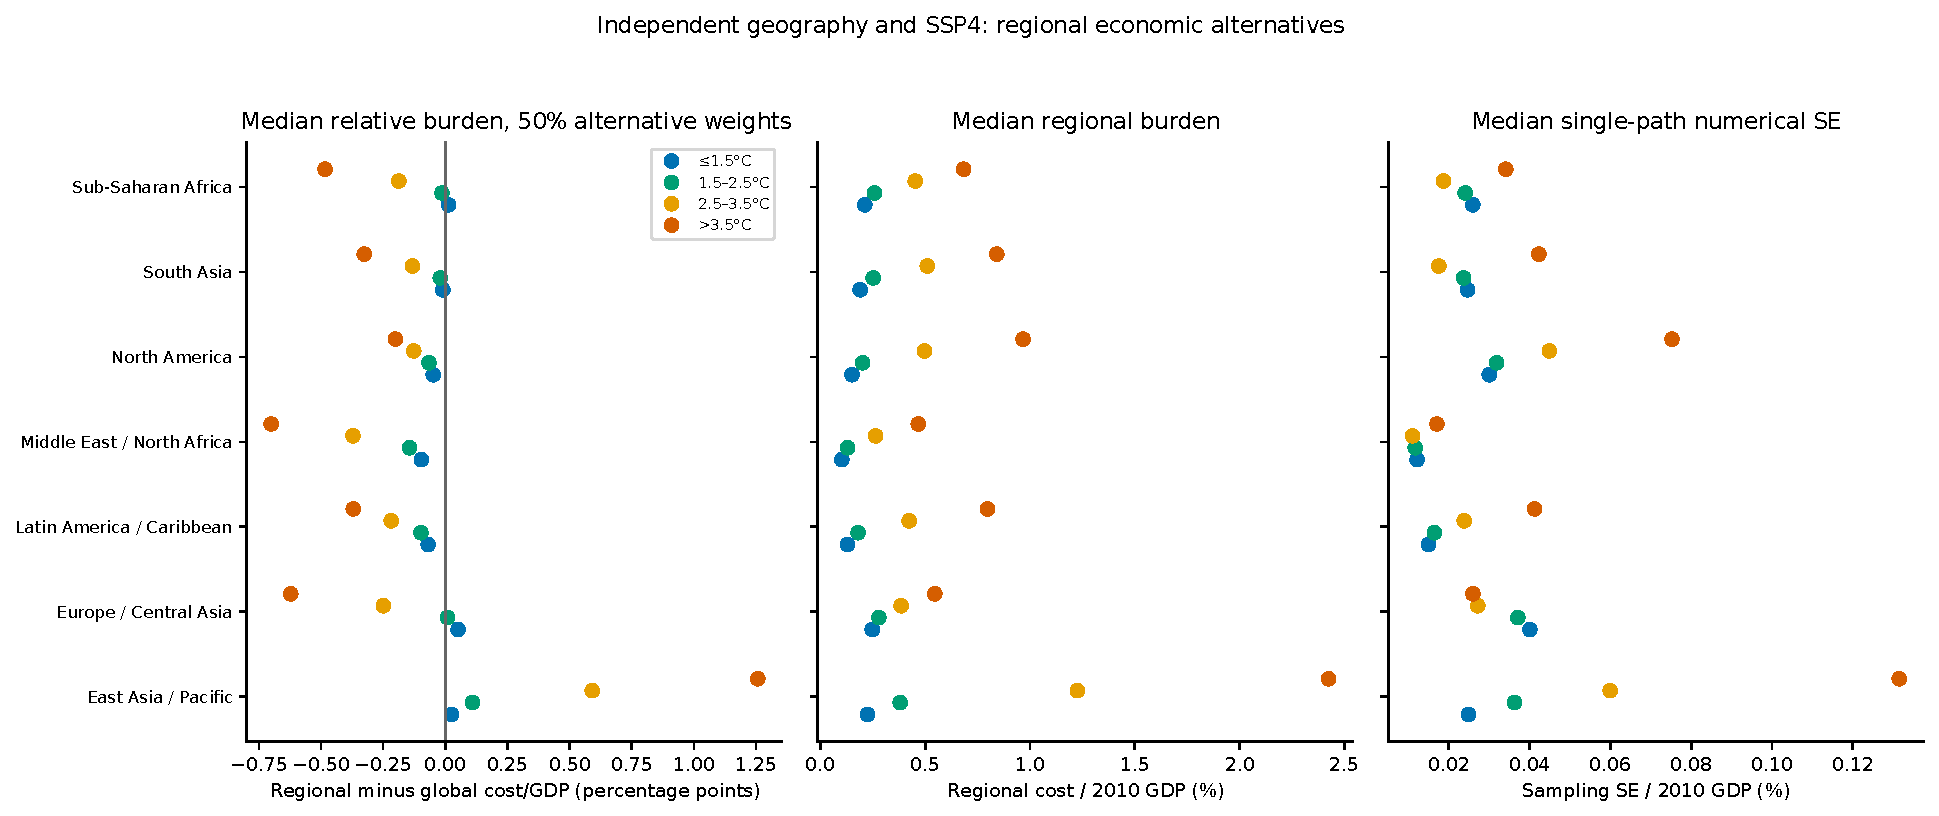
\includegraphics[width=\linewidth]{figures/coupled_coastal_regional_alternative.pdf}
\caption{Regional alternative for main Figure 3. Left: the median of each
member's regional-minus-covered-global cost/GDP ratio. Middle: median regional
incremental cost divided by 2010 GDP. Right: median conditional single-path
coastal sampling SE on the same GDP scale. The last quantity is not the SE of
the median. Symbols distinguish warming categories; the highest category has
only five members. Independent geography and economic accounting produce a
different regional pattern from the target's written findings.}
\label{fig:coupledregions}
\end{figure}

Under the fixed Antarctic point fit, 94 of 250 paths trigger rapid ice loss
before 2100, carrying 13.99\% of the alternative weight. Estimated median
planned movement is 79.93 million without triggering and 104.10 million with
triggering. Median conditional coast-sampling SE is 12.50 and 13.60 million,
respectively. The median paired difference from no-rise planned movement is
8.31 versus 32.48 million. These are movement counts under optimal modeled
policies, including initialization; they are neither counts of unique persons
nor forecasts of actual migration. Conditional association is not a causal
estimate of the Antarctic trigger, since triggering covaries with warming.

\begin{figure}[htbp]
\centering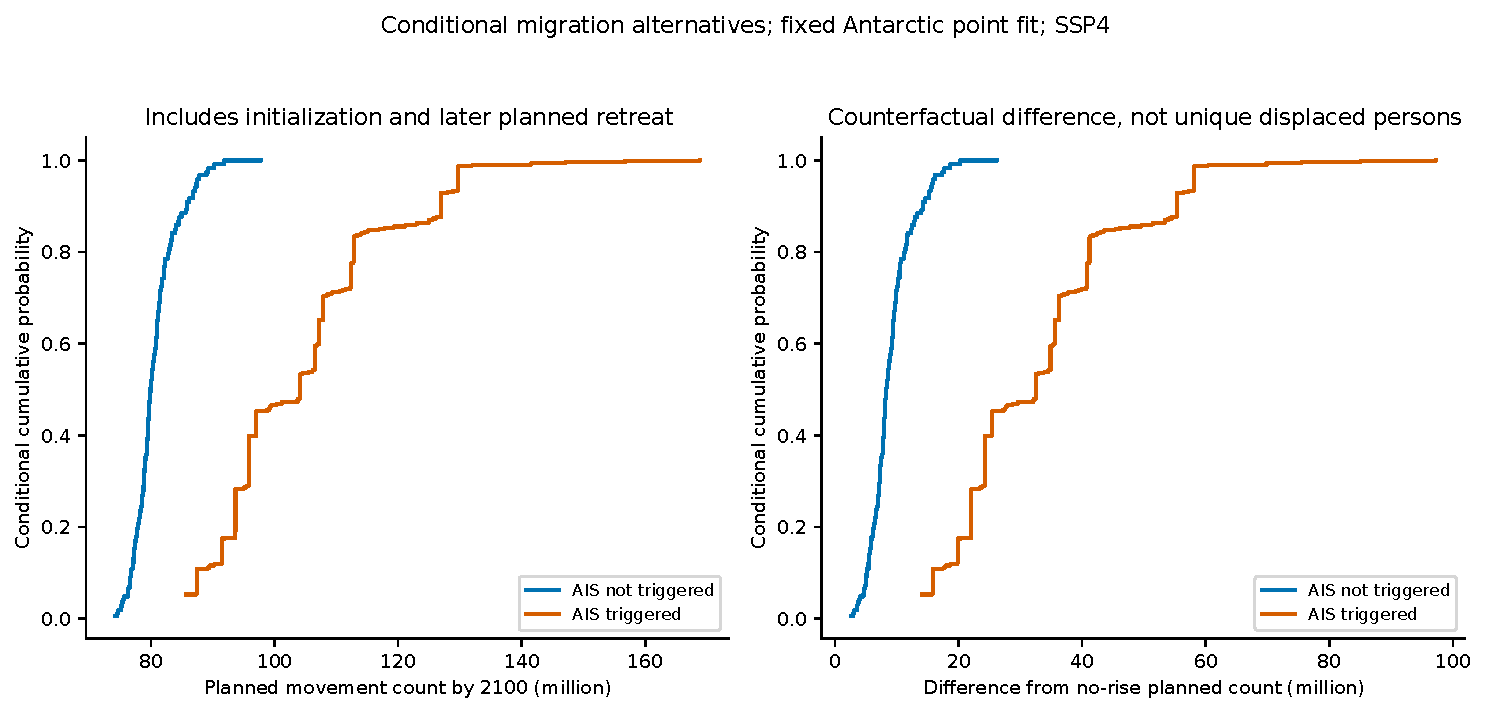
\includegraphics[width=\linewidth]{figures/coupled_coastal_migration_alternative.pdf}
\caption{Planned movement alternatives for supplementary Figure 10. The
empirical weighted distributions condition on whether the fixed Antarctic model
triggers by 2100. Left: all planned relocation, including initial adaptation.
Right: the paired difference from the no-rise planned count, which can be
negative when the optimal policy changes. These estimated distributions omit
target socioeconomic parameter uncertainty and are subject to the separately
reported coastal sampling error.}
\label{fig:coupledmigration}
\end{figure}

The alternative weighted 95th-percentile cost threshold is 0.597 trillion
2019 PPP. Its retained upper-tail members include one category-2 path, 48
category-3 paths and all five category-4 paths. No retained path exceeds the
target's literal 2.7 trillion threshold even after the CPI-only conversion.
Neither observation establishes a zero population probability: the target
threshold uses different units and accounting, and the high-warming tail is
poorly resolved.

\begin{figure}[htbp]
\centering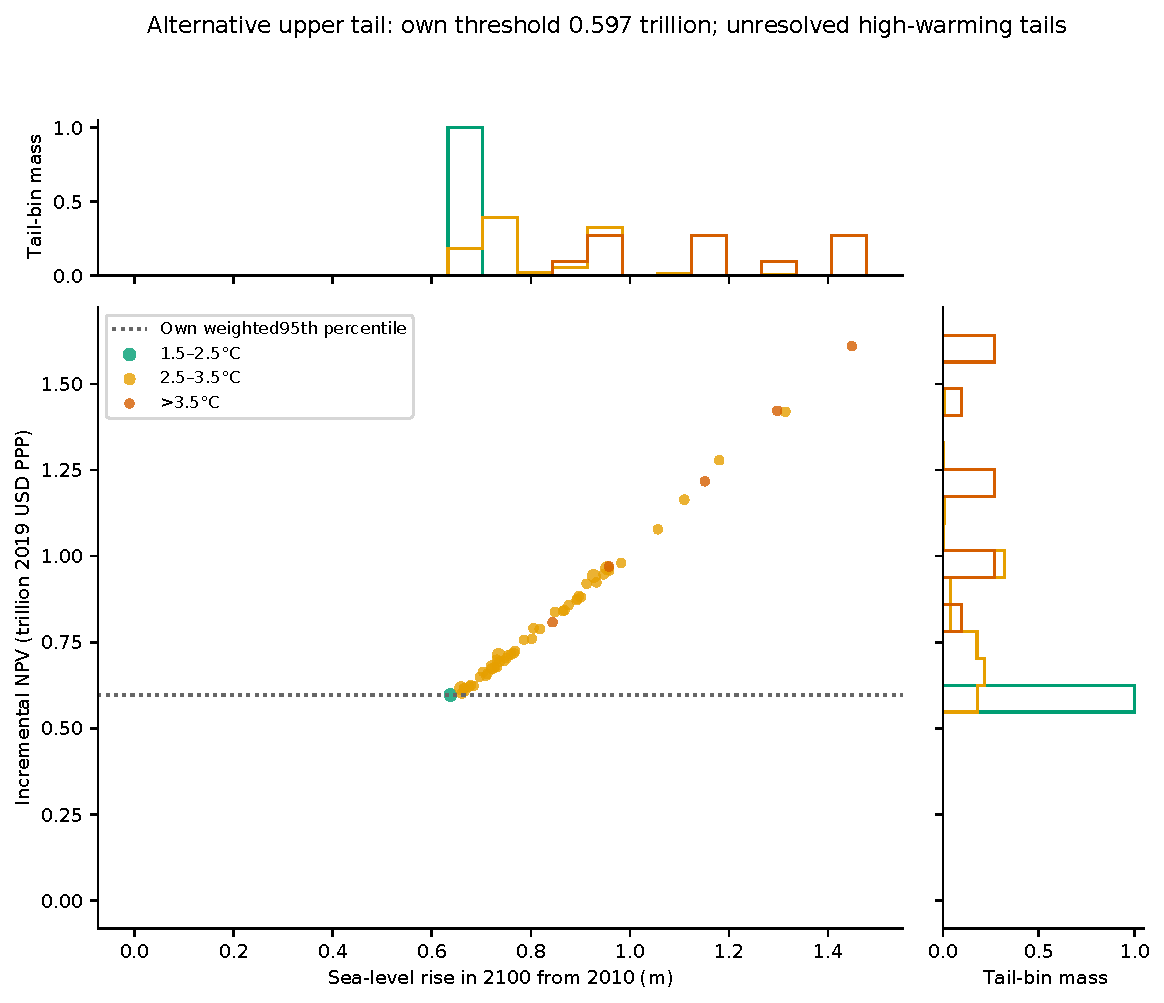
\includegraphics[width=.9\linewidth]{figures/coupled_coastal_tail_alternative.pdf}
\caption{Upper-tail alternative corresponding to supplementary Figure 7,
using the independent distribution's own weighted 95th-percentile threshold.
Empirical marginals normalize within each retained tail category. The plot
uses the same sea-level datum and cost conventions as
Figure~\ref{fig:coupledjoint}; it does not replace the target's 2.7 trillion
2010 USD selection. Tail category sizes and coastal sampling errors limit its
interpretation.}\label{fig:coupledtail}
\end{figure}
\subsection{Cost-baseline sensitivity}
The written CIAM lineage subtracts initial-interval calibration costs, whereas
the alternative above subtracts an independently optimized no-rise trajectory.
These operations need not agree. A six-path pilot holds the annual policies
fixed and separately retains gross costs, removes the 2010 payment, removes
all 2010--2019 payments, or subtracts the full no-rise trajectory.
The complete 9,531-coast no-rise present value is 1.958 trillion 2019 USD PPP.
Adding this known constant to the four baseline-subtracted medians gives
2.166, 2.249, 2.622 and 3.175 trillion. Thus the accounting convention can
reverse the sign of an apparent cost-level difference; gross costs are not
an alternative claim of agreement with the publication.

We also reject a literal annual interpretation that repeatedly subtracts the
2010 payment. That payment contains one-off investments; treating it as a
recurring reference rate produces values as low as $-44.23$ trillion.
The diagnostic exposes an invalid translation between annual investments and
decadal reference costs. It is not retained as a physical cost model.

\begin{figure}[htbp]
\centering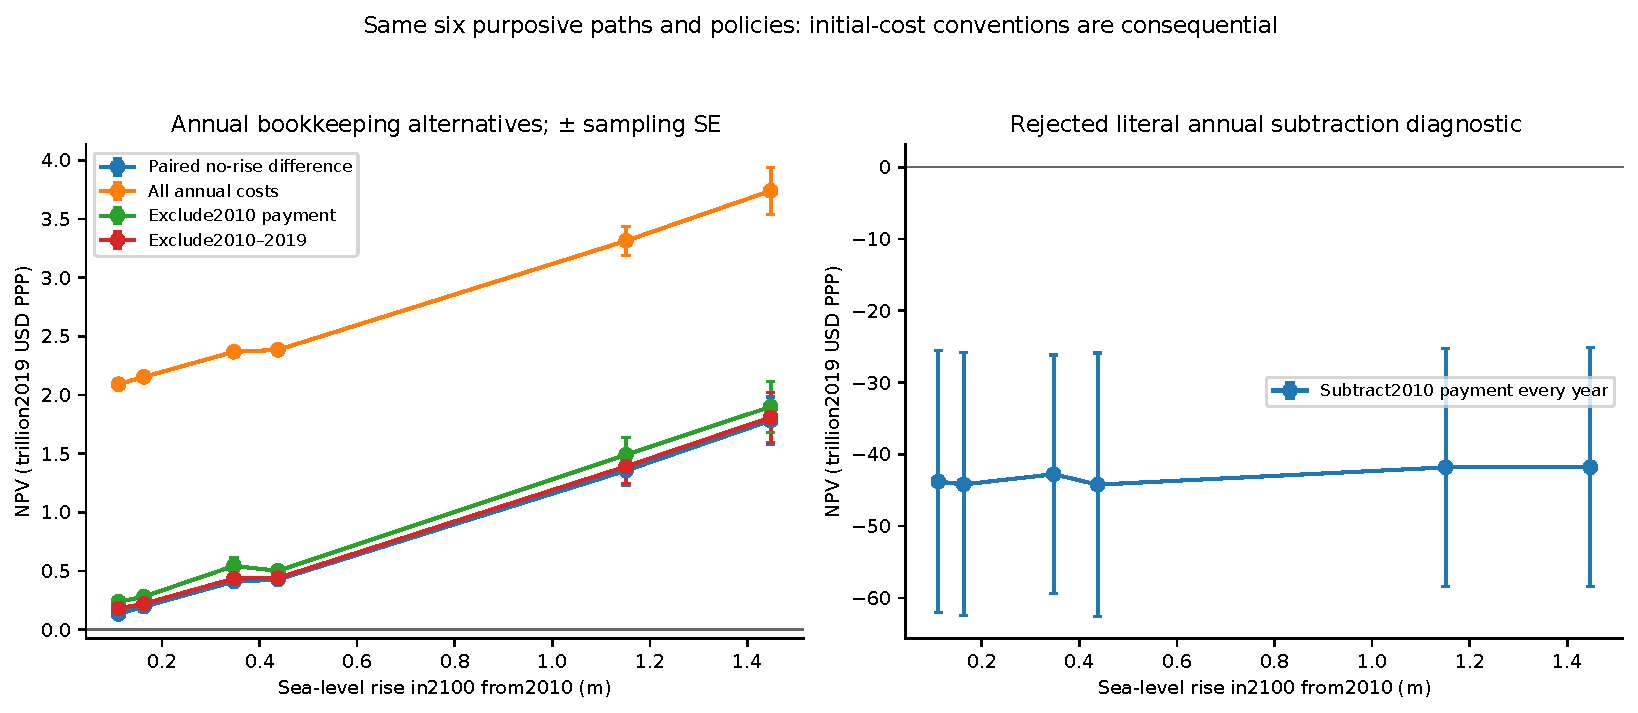
\includegraphics[width=\linewidth]{figures/coastal_accounting_sensitivity.pdf}
\caption{Accounting alternatives for six purposively selected paths and
four coastal draws per region. Left: different removals of initial or no-rise
costs, with conditional sampling SE. Gross totals use the known complete
no-rise sum as an additional control. Right: a rejected repeated subtraction
of a one-off initial payment. None of these conventions is asserted to recover
the target decadal spin-up accounting.}
\end{figure}
\subsection{Finite-ensemble and geographic sampling tests}
Supplementary Figures 1 and 2 ask whether the cost distributions depend on the
number of retained climate states. We test that question within the alternative
ensemble without claiming the target's 5,000 versus 4,000 comparison or its
202 members per warming category. Five hundred independent subsamples retain
200 of the 250 states, preserving the total weight of each emissions stratum.
The category-4 median difference has a 5th--95th range of
$-0.247$ to $+0.205$ trillion 2019 PPP. The category-2 upper quantile also
changes substantially: the median difference in its 95th percentile is
$+0.145$ trillion. Such behavior is incompatible with a claim that all tails
are converged.

A second test selects five distinct states per warming category. Its apparently
zero category-4 variability merely retains all five available states. The
category-3 median difference ranges from $-0.279$ to $+0.278$ trillion across
subsamples. Separately, nested coastal probability samples increase from four
to eight to sixteen draws per region. Increasing eight to sixteen changes the
four cost medians by $-0.0050$, $-0.0048$, $+0.0052$ and $-0.0400$ trillion.
These are dependent numerical samples, not independent posterior replications.
Neither this comparison nor a reduced conditional sampling SE establishes
convergence of the climate distribution or its rare-event probabilities.

\begin{figure}[htbp]
\centering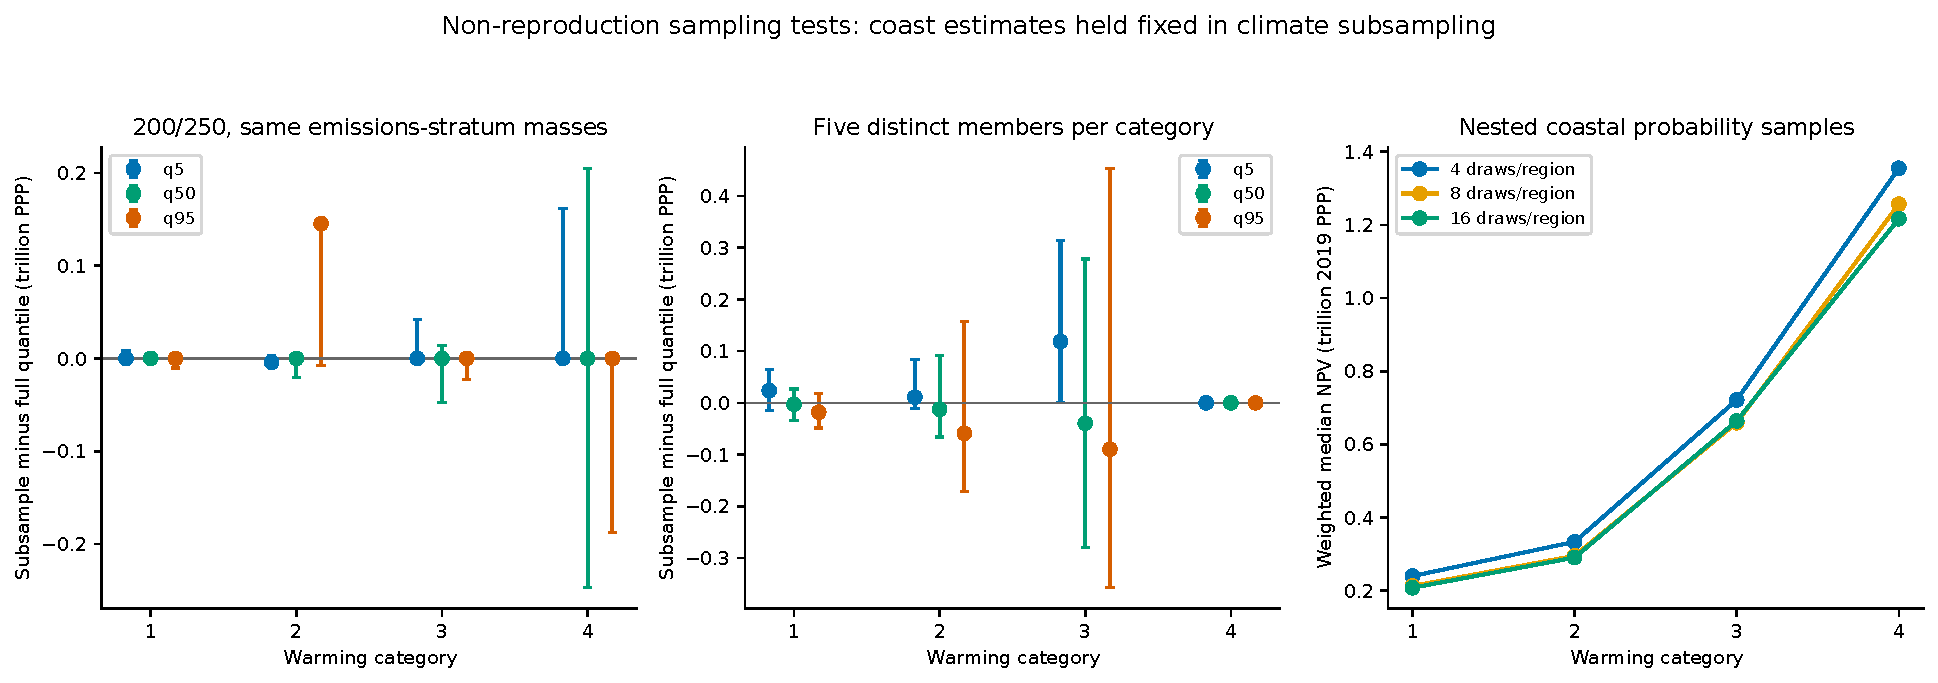
\includegraphics[width=\linewidth]{figures/coupled_sampling_sensitivity.pdf}
\caption{Alternatives addressing supplementary Figures 1 and 2. Left and
middle: median changes across 500 subsamples, with their 5th--95th ranges.
Coastal cost estimates are held fixed when subsampling climate states. Right:
conditional cost medians under nested coastal samples. The zero fourth-category
range in the equal-size test is a finite-population identity, not evidence of
convergence.}
\end{figure}

\subsection{Socioeconomic scenario, horizon and income contrasts}
A matched SSP2 calculation uses the same 250 climate--sea-level states and the
same eight coastal draws per region as a separately aggregated SSP4 calculation.
It evaluates 14,750 state--coast combinations after twelve pilot quadrature and
policy checks pass. The comparison isolates the scenario change within the
alternative geography, monetary units and annual accounting. East Asia and the
Pacific remains above the global cost/GDP burden in the high-warming categories;
the broader target Global South pattern is still not reproduced.

Six purposively selected paths test assumptions separately. SSP2 increases their
estimated global incremental costs by 0.66--1.78\% relative to SSP4. Extending
the horizon through 2150 increases costs by 4.40--33.18\% when post-2100
population and income are frozen. Continuing their final growth rates gives
4.38--33.01\%. These are two transparent extrapolations, not recovered
post-2100 socioeconomic specifications. Geometric interpolation between the
provider's nodes changes these six costs by less than 0.10\%. The results show
that horizon and initial-cost accounting deserve more attention than within-node
interpolation in these cases; they do not rank sensitivities for the population
of possible states.

\begin{figure}[htbp]
\centering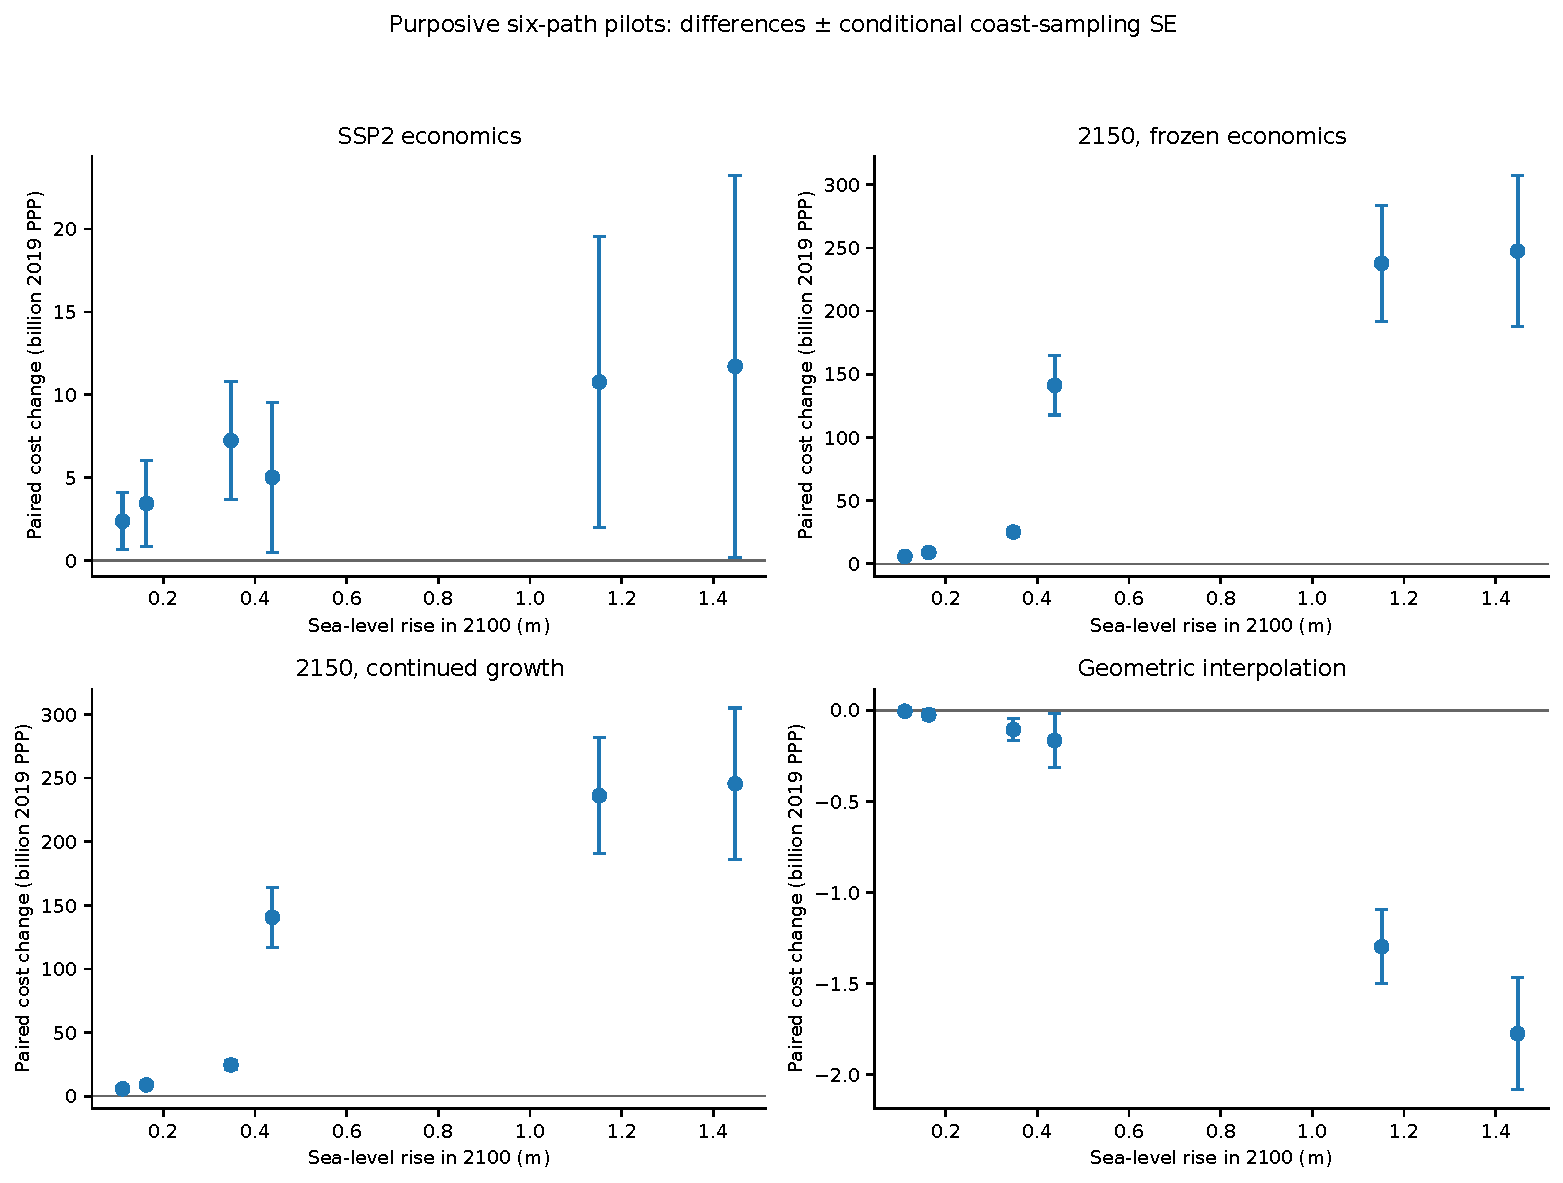
\includegraphics[width=\linewidth]{figures/coastal_assumption_pilots.pdf}
\caption{Paired six-path sensitivities. Error bars give conditional coastal
sampling SE of each difference. The horizon extensions retain the same
first-period policy rule and independently optimize each no-rise baseline.
They are explicit alternatives to unresolved target conventions.}
\end{figure}
\begin{figure}[htbp]
\centering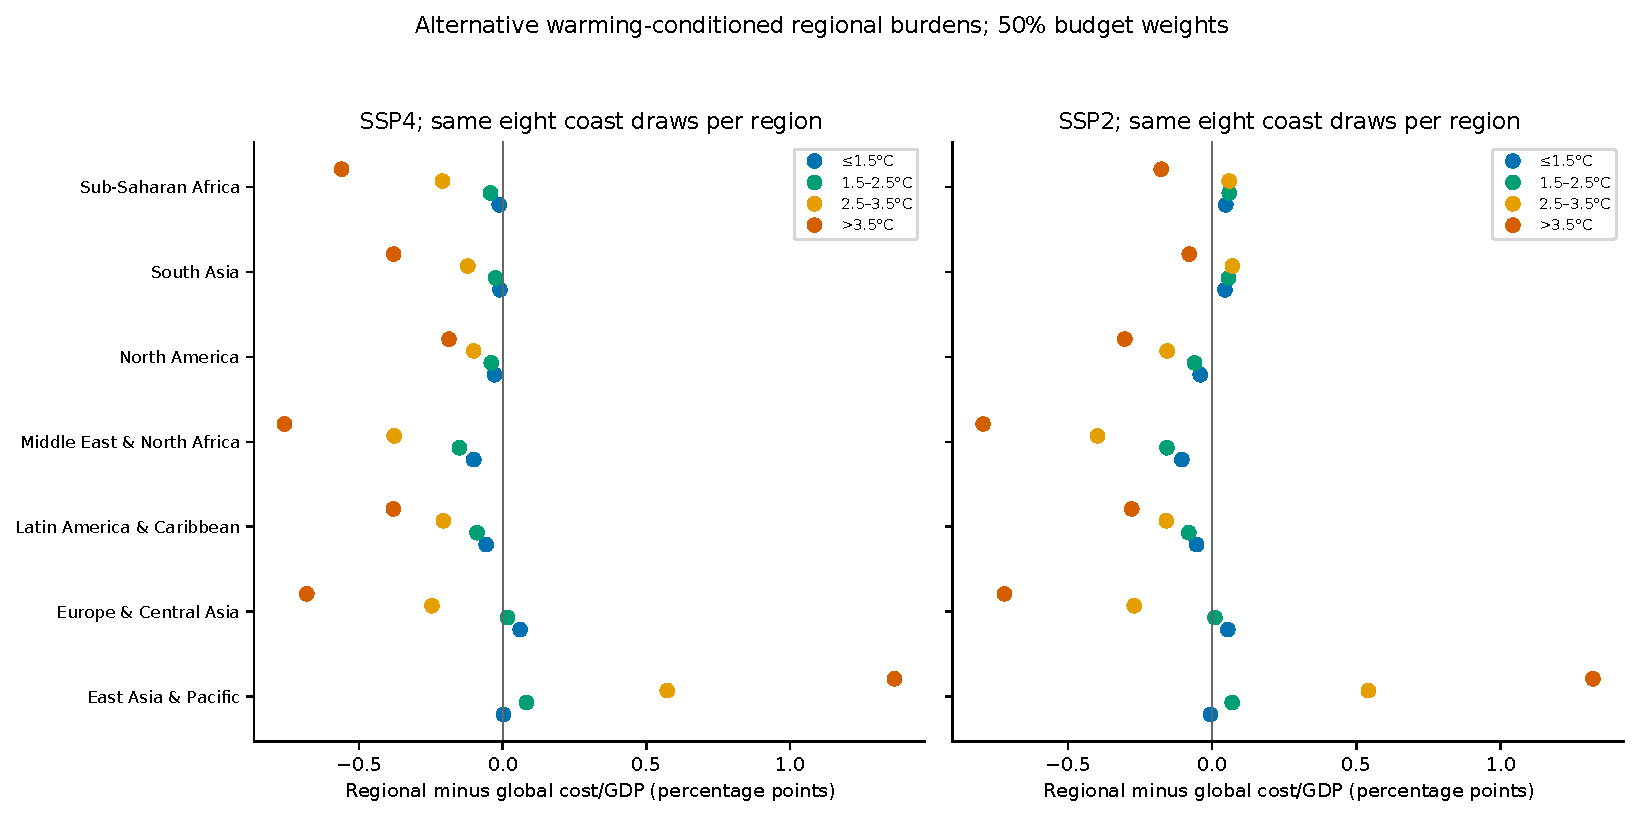
\includegraphics[width=\linewidth]{figures/coupled_ssp_comparison.pdf}
\caption{Supplementary Figure 8 alternative. Both scenarios use the same
250 climate states, eight coastal draws per region and alternative 50\% budget
weights. Points show the median regional-minus-global cost/GDP burden. The
panels compare socioeconomic inputs within the reconstruction; neither is a
published-result reproduction.}
\end{figure}

For supplementary Figure 9, the explicit contrast is SSP4 minus SSP2 of the
change between category-3 and category-2 median regional cost/GDP. The income
contrast is SSP4 minus SSP2 regional 2100 GDP per person. Regional populations
combine independent 2010 observations with provider scenario growth factors;
the least complete region covers 80.5\% of its reference population. Across
seven regions, the descriptive slope is 0.00219 percentage points per thousand
2019 PPP dollars, with $R^2=0.664$. The caption's precise target contrast,
coverage, cost inputs and monetary convention remain unmatched. Correlated
coastal sampling errors and seven aggregated observations preclude treating
this regression as a causal result or a validated target coefficient.

\begin{figure}[htbp]
\centering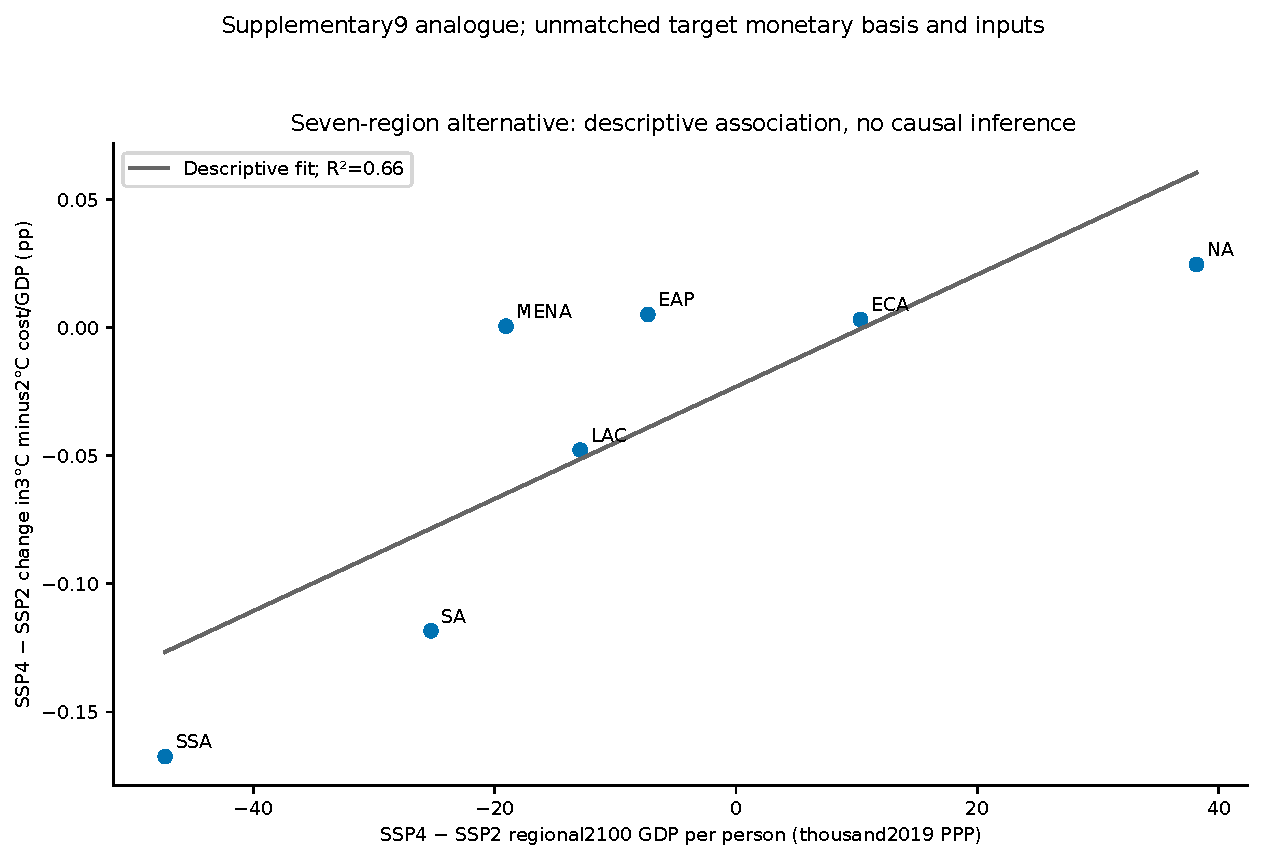
\includegraphics[width=.88\linewidth]{figures/coupled_regional_income_alternative.pdf}
\caption{Explicit interpretation of the supplementary Figure 9 comparison.
The line is a descriptive least-squares fit to seven alternative regional
contrasts. No significance test or causal interpretation is assigned.}
\end{figure}
